%% ============================================================
%% 分片 29：原文第 10 节「The Bogomolny Equations And The Space Of Hecke Modifications」（原文 glshort.tex 起于第 8120 行）
%% 由 tools/harvmac2tex.py 从 arXiv 源码（hep-th/0604151v3）自动生成。
%% 只译英文散文；公式、编号、\label、\cite 一律不改。
%% ============================================================

\subsection{Operator Product Expansion Of 't Hooft Operators}

\label{sec:opprod}

Let us write the tensor product of representations of $^L\negthinspace G$ as
% 式 (10.21)
\setcounter{equation}{20}
\begin{equation}\label{eq:yurgo}
^L\negthinspace R\otimes {}^L\negthinspace
R'=\bigoplus_{\alpha\in \EUR}\left(N_\alpha \otimes{}^L\negthinspace R_\alpha\right).
\end{equation}

Here $N_\alpha$ is the vector space $N_\alpha={\rm Hom}_G({}^L\neg R\otimes {}^L\neg{R'},{}^L\neg
R_\alpha)$, where ${\rm Hom}_G$ is the space of $G$-invariant linear transformations. The set $\EUR$
consists of
 the representations for which $N_\alpha$ is nonzero.
It is
convenient to also write $n_\alpha$ for the integer which is the dimension of the vector space
$N_\alpha$.

As we discussed in section 第~\ref{sec:lineop}~节, the tensor product of representations is precisely mirrored
in the operator product expansion of Wilson operators.  In eqn.  \eqref{eq:tryo}, we wrote the operator
product expansion for Wilson {\it loop} operators in terms of $c$-number coefficients $n_\alpha$.
However, for a static Wilson {\it line} operator, which we regard as part of the problem
of quantization, rather than an operator acting on quantum states, we can write a closely related and
more precise statement:
% 式 (10.22)
\setcounter{equation}{21}
\begin{equation}\label{eq:docus}
W({}^L\neg R,p)\cdot W({}^L\neg\tilde R,p')\to
\bigoplus_{\alpha\in\EUR}\left(N_\alpha\otimes W({}^L\neg
R_\alpha,p')\right).
\end{equation}

We are here taking the gauge group to be $^L\neg G$, and $p$ and $p'$ are the positions of the static
Wilson operators.
\eqref{eq:docus}\ is a recipe for constructing the quantum Hilbert space in the presence
of two Wilson operators labeled by $^L\neg R$ and $^L\neg R'$, as a direct sum of contributions;
each contribution is the tensor product with a vector space $N_\alpha$ of the quantum Hilbert space
obtained by quantization in the presence of a single Wilson operator labeled by $^L\neg R_\alpha$.  The basis
for the statement \eqref{eq:docus}\ is that the effect of a static Wilson operator in the quantum theory is
to introduce an external charge in the appropriate representation.  If there are two Wilson static
Wilson operators, there are  two external charges; after decomposing the tensor product of the
appropriate representations in a direct sum of irreducibles, one arrives at \eqref{eq:docus}.

From $S$-duality, we expect the corresponding operator
product expansion of 't Hooft line operators to take the same form
% 式 (10.23)
\setcounter{equation}{22}
\begin{equation}\label{eq:zurgo}
T({}^L\negthinspace R,p)\cdot T({}^L\negthinspace
R',p')\to \bigoplus_{\alpha\in \EUR}\left(N_\alpha \otimes T({}^L\negthinspace
R_\alpha,p')\right).
\end{equation}

As  in section 第~\ref{sec:lineop}~节, even without $S$-duality,  since the 't
Hooft operators are the only line operators at $\Psi=0$, a
relation such as \eqref{eq:zurgo}\ must hold with some set $\EUR$ of
representations (which depends on $^L\negthinspace R$ and
$^L\negthinspace R'$) and some vector spaces $N_\alpha$. Moreover,
simple arguments suffice to determine the set $\EUR$, which
depends on $^L\negthinspace R$ and $^L\negthinspace R'$. So the
problem is to describe the  $N_\alpha$.

If we specialize to the case of ordinary 't Hooft loop operators which may act on quantum states (as
opposed to static line
operators that modify the definition of the quantum Hilbert space), the coefficients in the operator
product expansion are ordinary $c$-numbers $n_\alpha$ rather than vector spaces $N_\alpha$.
One way to make this specialization is to take the ``time'' direction to be a circle.  This leads
to a trace in all of the quantum Hilbert spaces, and the vector space $N_\alpha$ is replaced by its
integer dimension $n_\alpha$.  The static 't Hooft line operators become circular 't Hooft loop operators
(which can act on quantum states if we interpret a different direction as the ``time'' direction
for quantization), and we learn that the operator product expansion coefficients
of 't Hooft loop operators, or of any loop operators in a topological field theory, are integers.

To make the point in a slightly different way, let us go back to the case of Wilson operators.
A closed Wilson loop operator is defined via the trace of the holonomy.
Taking the trace replaces a vector
space by its dimension.  But an open Wilson operator (the important example for us is a static Wilson
line operator) is defined in terms of the holonomy itself,
regarded as an operator on a vector space.  In decomposing the tensor products of such operators,
the ``coefficients'' are vector spaces $N_\alpha$, not integers $n_\alpha$.  For some purposes,
the distinction is not important and one can replace $N_\alpha$ by its dimension.

\par\medskip{\it Some Useful Branes}

Once the scene is properly set, the determination of the
$N_\alpha$ is a consequence of a mathematical theory that originated with
Lusztig's work \cite{ref98}\ on the relation of multiplicities in tensor products
of irreducible representations of $G$ to the convolution
of intersection cohomology complexes of affine Schubert varieties on $^L\neg G$,
and was further refined by Ginzburg \cite{ref96}\ and Mirkovic and Vilonen \cite{ref97}\
to an equivalence of tensor categories.  In physical terms, this refinement is related to
a description of the operator product expansion of 't Hooft operators in which the ``coefficients''
are vector spaces $N_\alpha$ (as in our equation \eqref{eq:zurgo}), as
opposed to a more conventional description in which only closed loop operators are considered and
the $N_\alpha$ are replaced by their integer dimensions $n_\alpha$ (as in our equation \eqref{eq:tryo}).
We will set the context for the
analysis, get as far as we can with purely physical reasoning, and
then attempt to elucidate the mathematical theory.

\begin{figure}[htbp]
\centering
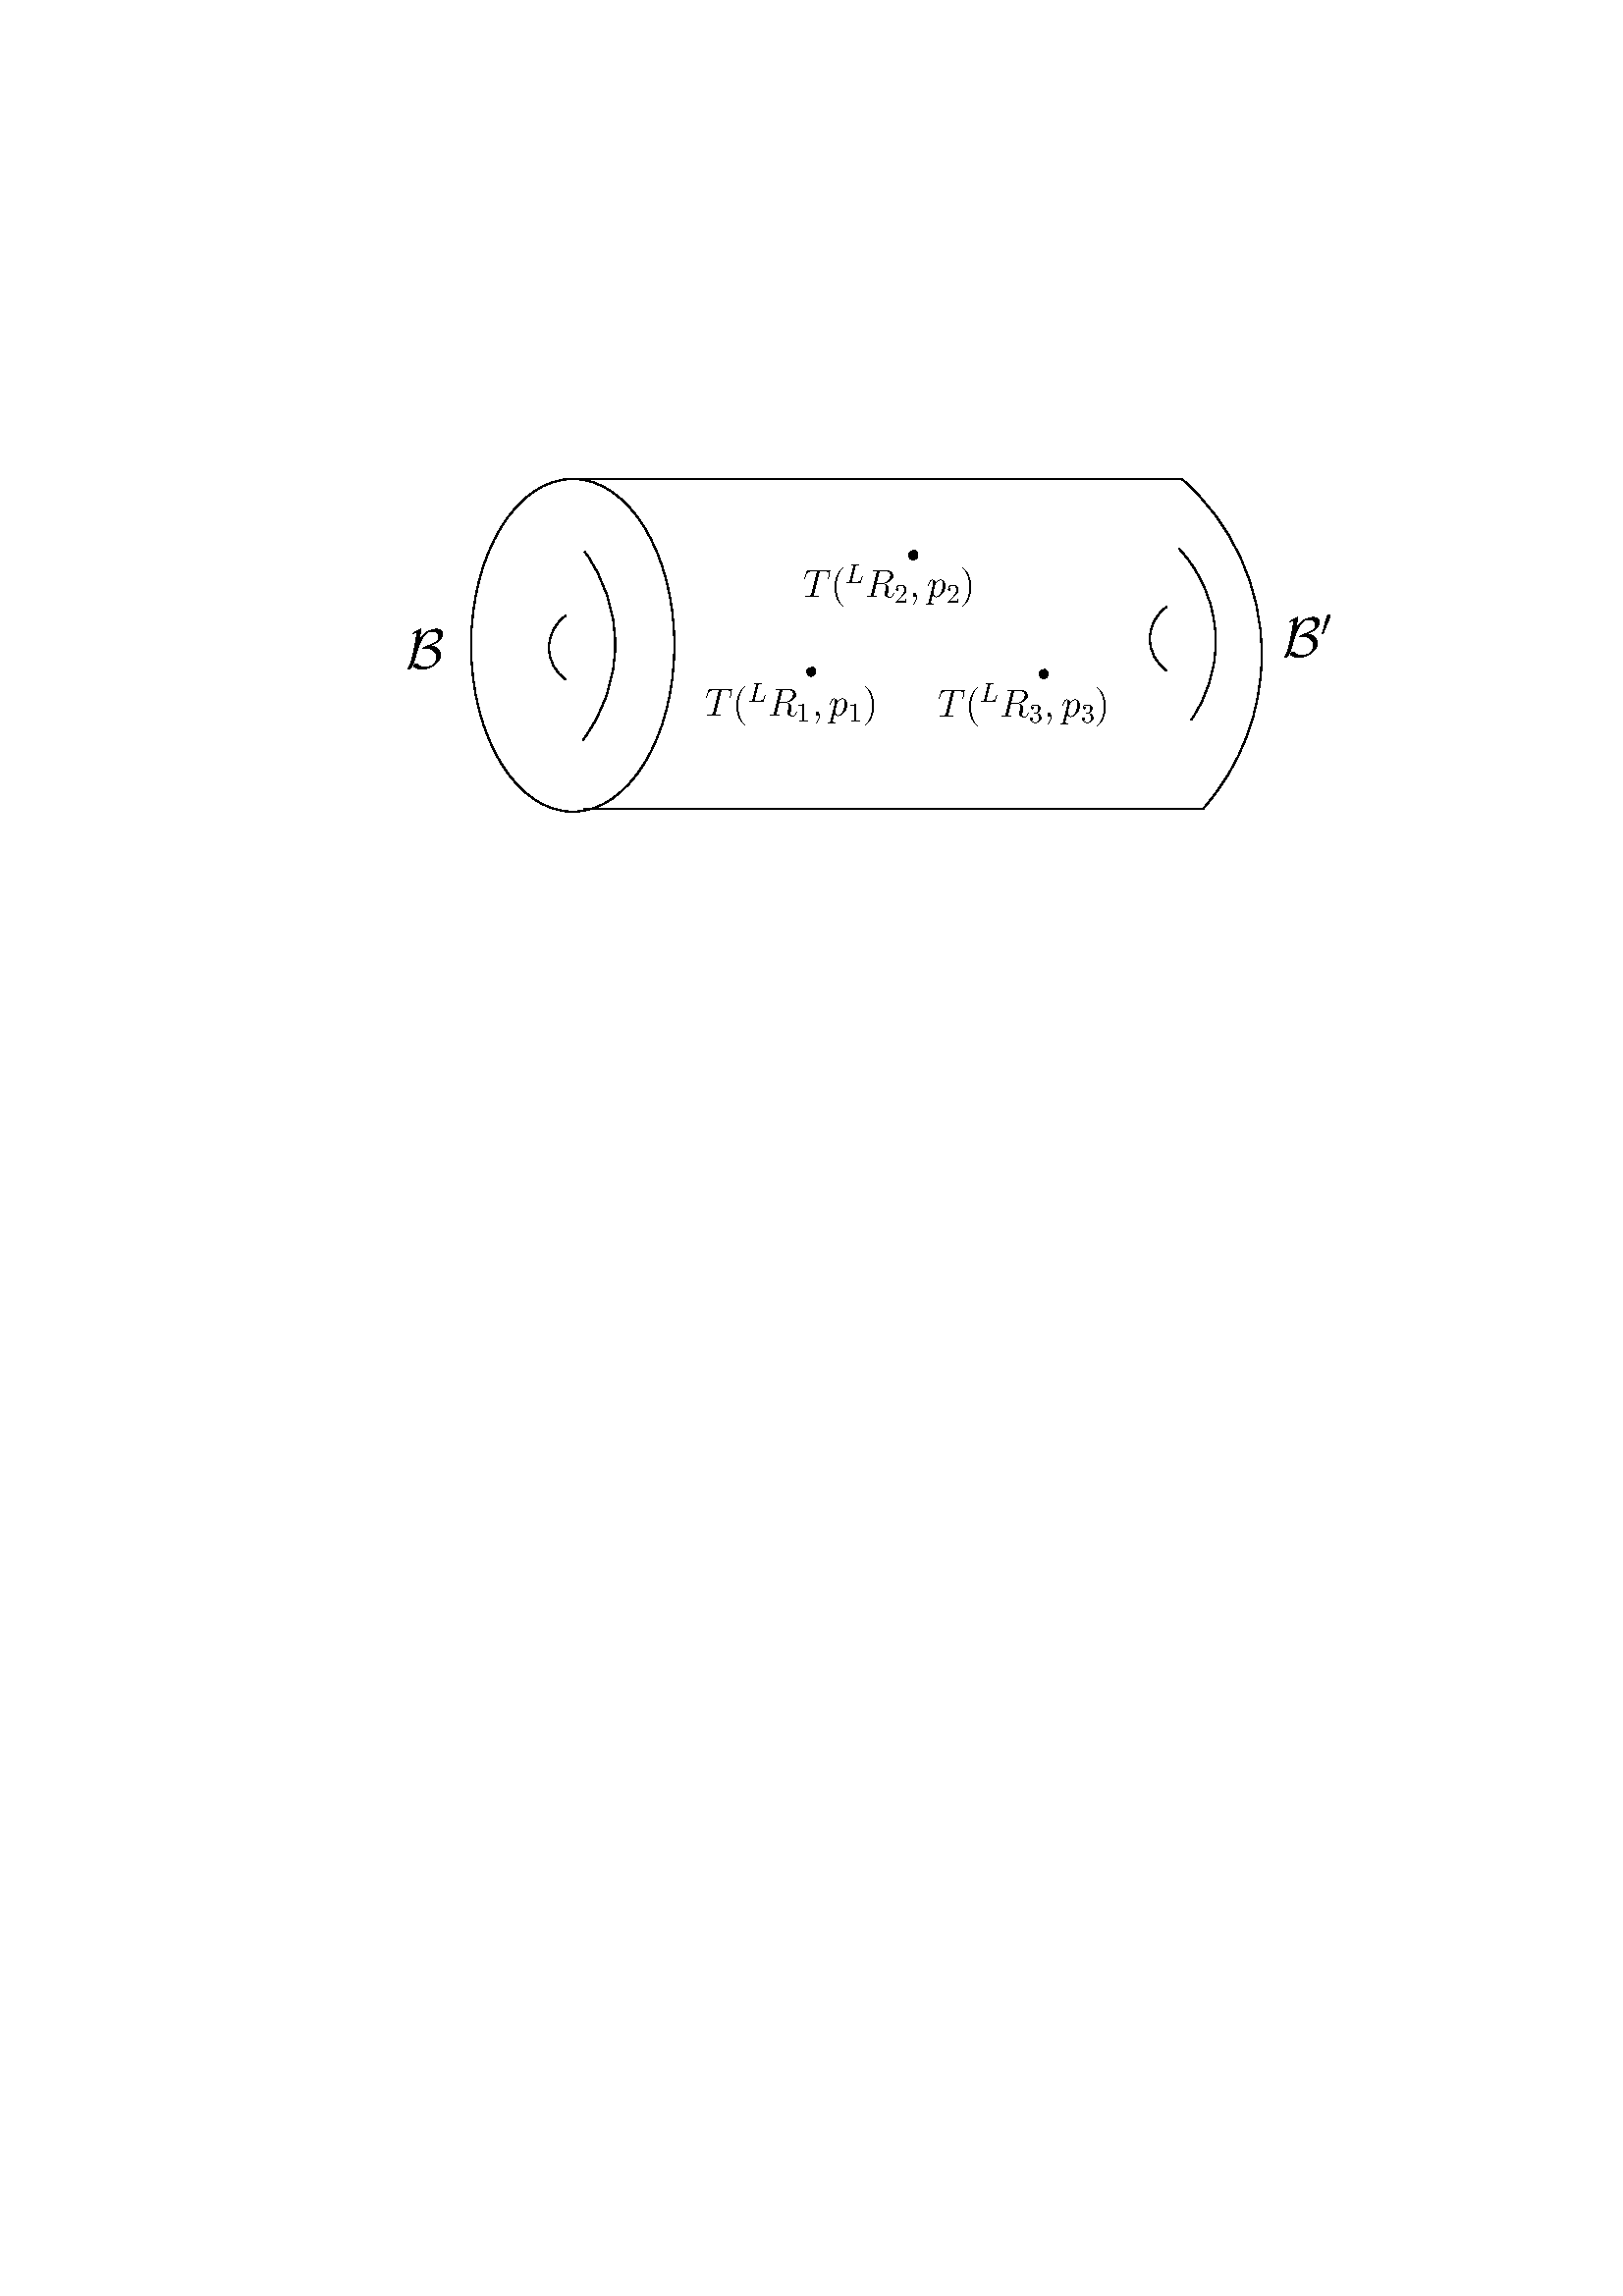
\includegraphics[width=0.75\linewidth]{figures/gla7-8.png}
\caption{Insertion of several 't Hooft operators $T({}^L\negthinspace R_i,p_i)$, with a brane ${\cal B}$ on the left that specifies an ``initial'' bundle $E_-$, and a brane ${\cal B}'$ on the right that sets $\varphi=0$.（原文 Fig.~19）}
\label{fig:xitampo}
\end{figure}

 To determine the $N_\alpha$, it suffices to consider any convenient and suitably rich
class of computations in which static 't Hooft operators play a role.
For this, we consider two or more 't Hooft operators in our
familiar three-manifold $W=I\times C$ and with suitable branes
${\cal B}$ and ${\cal B}'$ chosen at the two ends. We want to pick
branes that will simplify the computation.

't Hooft operators preserve supersymmetry of type $(B,A,A)$, so it
is most natural to choose ${\cal B}$ and ${\cal B}'$ to be branes
of that type.  For this, we can take ${\cal B}$ and ${\cal B}'$ to
be supported on subvarieties $U$ and $U'$ of Hitchin's moduli
space $\MH$ that are holomorphic in complex structure $I$ and
Lagrangian with respect to the symplectic form $\Omega_I$ that is
of type $(2,0)$ in this complex structure. (More briefly, $U$ and
$U'$ are complex Lagrangian submanifolds in complex structure
$I$.) We endow $U$ and $U'$ with  trivial Chan-Paton line
bundles.

We take $U$ to parametrize Hitchin pairs $(E,\varphi)$, where we
require $E$ to have a specified holomorphic type $E_-$ and
arbitrary $\varphi$. We require $E_-$ to be stable, but otherwise
the choice of $E_-$ does not matter.   And we take $U'$ to
parametrize pairs $(E,0)$ with any $E$ but with $\varphi=0$.

The first point is that $U$ and $U'$ intersect transversely at a
single point, corresponding to the Higgs bundle $(E_-,0)$. Moreover,
$U$ and $U'$ are complex symplectic manifolds in complex structure
$I$, so ${\cal B}$ and ${\cal B}'$ are branes of type $(B,A,A)$.

Finally, we have chosen ${\cal B}$ and ${\cal B}'$ so that the
space of supersymmetric configurations with these boundary
conditions and with some 't Hooft operators included is precisely
the familiar moduli space ${\EUZ}({}^L\negthinspace R_1,p_1;\dots;{}^L\negthinspace R_k,p_k)$ of
solutions of the Bogomolny equations.

 A few subtleties go into this statement.
First of all, supersymmetric configurations in general have
$\varphi\not= 0$ and must be described using the extended
Bogomolny equation that we described at the outset of section
第~\ref{sec:thooftheckeop}~节, not the ordinary Bogomolny equations.  We have not
yet even analyzed the extended Bogomolny equations; this will be
the subject of section 第~\ref{sec:extbog}~节. When we do so, we will see that if
$\varphi$ vanishes at one end of $W$ -- and it does here, because
of the choice of $U'$ -- then $\varphi$ vanishes everywhere, and
the extended Bogomolny equations reduce to ordinary ones.

Second, in describing the branes ${\cal B}$ and ${\cal B}'$, we
only described the boundary conditions on the fields $(A,\varphi)$
of the sigma-model with target $\MH$.  The field $\phi_0$, which
is an important part of the Bogomolny equations, is present in the
gauge theory, but not in the sigma-model (except at singularities)
because in reduction to two dimensions it is ``massive.''  By
extending the analysis in section 第~\ref{sec:zapendix}~节, the branes ${\cal B}$
and ${\cal B}'$ can both be described in gauge theory \cite{ref26}, and
in that context it can be shown that the appropriate boundary
conditions for the field $\phi_0$ are the ones we use.

\par\medskip{\it The Space Of Physical States}

In the $A$-model, in the absence of instanton corrections (they
are absent here for reasons we discussed at the beginning of
section 第~\ref{sec:thooftheckeop}~节), the space of physical states is the
cohomology of the space of time-independent supersymmetric
configurations.  In fact, the $A$-model as understood physically
leads most naturally to de Rham cohomology.

In other words, with branes ${\cal B}$ and ${\cal B}'$, and 't
Hooft operators $T(^L\negthinspace R_i,p_i)$, the space of
physical states is the cohomology of our friend, the moduli space
$\bar\EUZ(^L\negthinspace R_1,p_1;\dots;^L\neg R_k,p_k)$ of solutions of the Bogomolny
equations with the appropriate singularities. As $\bar\EUZ$ is
generically singular, we need to explain here what kind of
refinement of de Rham cohomology is meant. But first let us just
formally state what sort of result we expect.

For every finite set of representations $^L\negthinspace R_i$,
$i=1,\dots,k$, the cohomology of the moduli space
$\bar\EUZ=\bar\EUZ(^L\negthinspace R_1,p_1;\dots;{}^L\neg R_k,p_k)$
 gives us a space of physical
states ${\cal H}({}^L\negthinspace R_1,{}^L\negthinspace
R_2,\dots,{}^L\negthinspace R_k)=H^*(\bar\EUZ)$.
Notice that because of the underlying four-dimensional
topological quantum field theory (TQFT), the choices of the points
$p_i$ do not matter.  To be more exact, the TQFT says that locally
in $p_i$ the space of physical states is independent of the $p_i$
(there is a flat connection\footnote{Moving the points is a special
case of changing the metric on $W$.  The change in metric is
trivial in the BRST cohomology, a fact which gives the flat
connection.} on the space of distinct points $p_i$). Since the
space of $n$-tuples in the three-manifold $W=I\times C$ is
simply-connected, there is also no room for monodromies, and thus
the $p_i$ are irrelevant. So we have labeled the space of physical
states ${\cal H}({}^L\negthinspace R_1,\dots,{}^L\negthinspace
R_k)$ just by the representations, not by the points.

Modulo questions about singularities, we do not really need
quantum field theory for this argument. In the case that the
representations $^L\negthinspace R_i$ are minuscule (and the $p_i$
are distinct), $\bar\EUZ(^L\negthinspace R_1,p_1;\dots;{}^L\neg R_k,p_k)$ is a family
of smooth manifolds. The cohomology of such a family is locally
constant, just as expected from the TQFT. In the general case with
singularities, we need to make sure to use a refinement of de Rham
cohomology in which this sort of argument is valid.  The property
of $\bar\EUZ(^L\negthinspace R_1,p_1;\dots;{}^L\neg R_k,p_k)$ that makes this possible
is that, although it is singular, its singular structure is
completely independent of the $p_i$.  The singularities come from
degenerations of individual Hecke transformations (or monopole
bubbling at positions of individual 't Hooft operators),
independent of the positions of the others.

Now the operator product expansion says that we can replace a
product of 't Hooft operators $T(^L\negthinspace R_1)\cdot
T(^L\negthinspace R_2)$ by a sum $\oplus_{\alpha\in \EUR}C_\alpha\otimes
T(^L\negthinspace R_\alpha)$, with some set $\EUR$ and some
vector spaces $C_\alpha$.  In the present context, for spaces of
physical states in the presence of the branes we have considered,
this means we must have a family of isomorphisms % 式 (10.24)
\setcounter{equation}{23}
\begin{equation}\label{eq:mitrox}
{\cal
H}({}^L\negthinspace R_1,{}^L\negthinspace
R_2,\dots,{}^L\negthinspace R_k)\cong\oplus_{\alpha\in
\EUR}\left(C_\alpha \otimes{\cal H}({}^L\negthinspace
R_\alpha,{}^L\negthinspace R_3,\dots,{}^L\negthinspace R_k)\right).
\end{equation}

Since the left hand side only depends on the unordered set of
representations $^L\negthinspace R_i$, the isomorphisms in
\eqref{eq:mitrox}\ are automatically compatible with associativity, that is
with taking repeated operator products to further reduce the
number of representations.

$S$-duality says that the set $\EUR$ and vector spaces $C_\alpha$
should be the ones that arise in the tensor product of
representations of $^L\negthinspace R$:
% 式 (10.25)
\setcounter{equation}{24}
\begin{equation}\label{eq:omigron}
^L\negthinspace R_1\otimes {}^L\negthinspace
R_2=\oplus_{\alpha\in \EUR}\left(N_\alpha\otimes{} ^L\negthinspace R_\alpha\right).
\end{equation}

We actually can be much more specific if we recall that\footnote{These
assertions do not depend on the points $p_i\in W$, so we omit
them.} ${\cal H}({}^L\negthinspace R_1,^L\negthinspace
R_2,\dots,^L\negthinspace R_k)$ is the cohomology of
$\bar\EUZ({}^L\negthinspace R_1,{}^L\negthinspace
R_2,\dots,{}^L\negthinspace R_k)$  and
that topologically $\bar\EUZ({}^L\negthinspace R_1,{}^L\negthinspace
R_2,\dots,{}^L\negthinspace R_k)$ is a simple product
$\prod_{i=1}^k\bar\EUZ({}^L\negthinspace R_i)$.  (And
$\bar\EUZ({}^L\negthinspace R_i)$ is the same as the compactified
space $\bar {{\EUY}}({}^L\negthinspace R_i)$ of Hecke
modifications of type ${}^L\negthinspace R_i$.)  The de Rham
cohomology of a product is the product of the cohomologies of the
factors, so we get % 式 (10.26)
\setcounter{equation}{25}
\begin{equation}\label{eq:kipro}
{\cal H}({}^L\negthinspace
R_1,{}^L\negthinspace R_2,\dots,{}^L\negthinspace
R_k)=\otimes_{i=1}^k {\cal H}({}^L\negthinspace R_i).
\end{equation}
 This
implies that \eqref{eq:mitrox}\ must really come from a family of
isomorphisms % 式 (10.27)
\setcounter{equation}{26}
\begin{equation}\label{eq:gitrox}
{\cal H}({}^L\negthinspace R_1)\otimes
{\cal H}({}^L\negthinspace R_2)=\oplus_{\alpha\in \EUR}N_\alpha\otimes
{\cal H}({}^L\negthinspace R_\alpha).
\end{equation}

Comparing \eqref{eq:omigron}\ to \eqref{eq:gitrox}, we see that the ${\cal
H}({}^L\negthinspace R_i)$ obey the same algebra of tensor
products as the $^L\negthinspace R_i$.  This suggests that there
is an isomorphism between ${\cal H}({}^L\negthinspace R_i)$ and
$^L\negthinspace R_i$ that produces the automorphism between the
two algebras. Indeed, it can be shown \cite{ref127} that this is the only way for the families of
finite-dimensional vector spaces $^L\negthinspace R_i$ and ${\cal
H}(^L\negthinspace R_i)$ to have the same algebra of tensor
products.  The isomorphism between ${\cal H}({}^L\negthinspace
R_i)$ and $^L\negthinspace R_i$ is unique up to conjugation by an
element  of $^L\negthinspace G$.

\par\medskip{\it Grading By Ghost Number}

Since $^L\negthinspace G$ certainly acts on the $^L\negthinspace
R_i$, in a way compatible with the tensor products, this means
that there is a corresponding action of $^L\negthinspace G$ on
${\cal H}({}^L\negthinspace R_i)$ (defined up to conjugation).
What this means is mysterious from a physical point of view, since
$^L\negthinspace G$ is not a symmetry of the full $A$-model of
gauge group $G$ at $\Psi=0$, but only of the particular piece of
it that we have looked at to analyze the operator product
expansion. (Things might become clearer if one could understand
the $S$-duals of the branes ${\cal B}$ and ${\cal B}'$ that were
used in the construction.) However, the full $A$-model does have
one symmetry that is relevant.

This is the ``ghost number'' symmetry ${\EUK}$, whose origin in
topological twisting of ${\EUN}=4$ super Yang-Mills theory was
explained in section 第~\ref{sec:twisting}~节.  In the $A$-model, the ghost
number is, roughly speaking, the degree or dimension of a
cohomology class.\footnote{For a Kahler target, the Hodge
decomposition $H^d(X)=\oplus_{p+q=d}\,H^{p,q}(X)$ gives a further
refinement  of the $A$-model, in general. However, this is not
relevant for our present discussion, as the cohomology of the
spaces  $\bar \EUZ({}^L\negthinspace R_1,\dots,{}^L\neg R_k)$ is all of type $(p,p)$.}
There is, however, one key subtlety.  For a complex manifold $X$
of complex dimension $n$, the degree of a differential form is
usually understood to run from $0$ to $2n$. But the space of
physical states of the $A$-model has a fermion conjugation
symmetry\footnote{The symmetry in question is two-dimensional CPT
symmetry.  It is an exact symmetry of the physical supersymmetric
sigma-model with $(2,2)$ supersymmetry and target $X$. On a
non-flat Riemann surface $\Sigma$, this symmetry is spoiled by the
topological twisting that defines the $A$-model.  But the space of
physical states is obtained by quantizing the sigma-model on the
flat manifold $\Bbb{R}\times S^1$, which is unaffected by the
twisting.} that exchanges a class of dimension $d$ with one of
dimension $2n-d$ and maps ${\EUK}\to -{\EUK}$. The ghost number of
a state that is related to a cohomology class of degree $d$ is
actually\footnote{ For completeness, let us note that if $X$ is a
Calabi-Yau manifold, then the $A$-model mapping from states to
operators involves a spectral flow that adds $\dim_{\Bbb{C}}(X)$
to ${\EUK}$.  So if $\psi$ is a class in the $d$-dimensional
cohomology of $X$, then the $A$-model state corresponding to
$\psi$ has ${\EUK}=d-{\rm dim}_{\Bbb{C}}(X)$, but the
corresponding operator ${\EUO}_\psi$ has ${\EUK}=d$. However, the
spaces $\bar \EUZ({}^L\negthinspace R_1,\dots,{}^L\neg R_k)$ are not Calabi-Yau,
and more importantly our discussion of branes and 't Hooft
operators refers to the physical states, not to corresponding
operators.} % 式 (10.28)
\setcounter{equation}{27}
\begin{equation}\label{eq:insno}
{\EUK}=d-{\rm dim}_{\Bbb{C}}(X).
\end{equation}

In the map from $^L\negthinspace R_i$ to ${\cal H}(^L\negthinspace
R_i)$, the symmetry ${\EUK}$ of the $A$-model  must correspond to
a derivation (that is, the generator of an automorphism) of the
tensor algebra of representations of $^L\negthinspace G$. Any such
derivation is actually an element of the complexified Lie algebra
$^L\negthinspace \frak{g}$. The element of $^L\negthinspace
\frak{g}$ corresponding to ${\EUK}$ is well-defined up to
conjugation.

For given $^L\negthinspace G$, one can find the right conjugacy
class by considering a specific example.  For example, for
$^L\negthinspace G=SU(N)$, consider the $N$-dimensional
representation $\VV$. The corresponding space of Hecke
modifications is $\bar {{\EUY}}(\VV)\cong \Bbb{CP}^{N-1}$, as we
learned in section 第~\ref{sec:spaceheck}~节. The de Rham cohomology of
$\Bbb{CP}^{N-1}$ is $N$-dimensional. The fact that this coincides
with the dimension of $\VV$ is an example of the correspondence
$^L\negthinspace R\leftrightarrow {\cal H}({}^L\negthinspace R)$.
$\Bbb{CP}^{N-1}$ has complex dimension $N-1$ and has cohomology in
dimensions $d=0,2,4,\dots,2N-2$. So the element of
$^L\negthinspace \frak{g}$ corresponding to ${\EUK}$  has
eigenvalues $N-1,N-3,N-5,\dots,-(N-1)$ in the representation
$\VV$: % 式 (10.29)
\setcounter{equation}{28}
\begin{equation}\label{eq:unosn}
\EUK=\left(\begin{matrix}N-1& &&& \\ & N-3 &&&\\ &&
N-5 &&\\ &&&\ddots & \\ &&&& -(N-1)\\\end{matrix}\right).
\end{equation}
 For
$^L\negthinspace G=SU(2)$, the conjugacy class of ${\EUK}$ is
simply % 式 (10.30)
\setcounter{equation}{29}
\begin{equation}\label{eq:mitlgo}
{\EUK}\cong\left(\begin{matrix}1 & 0 \\ 0 & -1
\\\end{matrix}\right).
\end{equation}

\par\medskip{\it Intersection Cohomology}

 A mathematical theory that was initiated by Lusztig \cite{ref98}, and
 later refined by   Ginzburg \cite{ref96}\ and Mirkovic and
Vilonen \cite{ref97}, in effect determines the ``coefficients'' in
the operator product expansion of 't Hooft operators. Describing
these results in detail is a task better left to others. Instead,
here we will try to express a few of the ideas in a language that
physicists might find illuminating.

 First of all, the cohomology theory used in this theorem is intersection cohomology
\cite{ref128,ref129}.
 Roughly speaking,
and modulo standard conjectures, the intersection cohomology of an
algebraic variety $X$ is the ${\Bbb{L}}^2$ cohomology of the
smooth part of $X$.  One considers square-integrable differential
forms on the smooth part of $X$. The intersection cohomology
$IH^*(X)$ is the cohomology of the exterior derivative operator
$d$ in the space of such square-integrable forms.  (It cannot
necessarily be expressed in terms of harmonic forms.)  To match
intersection cohomology with quantum field theory, it is useful to
make the same shift in dimensions that arises naturally in the
$A$-model: we define a grading of $IH^*(X)$ such that an ${\Bbb{
L}}^2$ cohomology class that is a $d$-form is considered to have
degree $\EUK=d-{\rm dim}_{{\Bbb C}}(X)$.

To be more precise, the ${\Bbb{L}}^2$ cohomology of the smooth
part of $X$ is the intersection cohomology of $X$ relative to its
standard intersection cohomology complex.  We might denote this
$IH^*(X,IC_X)$.  One also defines other intersection cohomology
complexes on $X$.  We will really only need the simplest
construction. If $Y\subset X$ is a subvariety, one defines an
intersection cohomology complex $IC_Y$ which is supported on $Y$
and such that $H^*(X,IC_Y)$ is the ${\Bbb{L}}^2$ cohomology of the
smooth part of $Y$, shifted in dimension by $-{\rm
dim}_{\Bbb{C}}(Y)$. Thus, $IC_Y$ is the standard intersection
cohomology complex of $Y$, but embedded in $X$ (and ``extended by
zero'' away from $Y\subset X$).

In the case of the spaces $\bar {{\EUY}}({}^L\bar w)$ of Hecke
modifications, the subvarieties of interest are the spaces $\bar
{{\EUY}}({}^L\negthinspace w_\alpha)$, where $^L\negthinspace
w_\alpha$ is a weight associated to $^L\negthinspace\,\bar w$. So
for each associated weight, one defines an intersection cohomology
complex $IC({}^L\negthinspace w_\alpha)$, supported on the
subspace of $\bar {{\EUY}}({}^L\bar w)$ on which monopole bubbling
has reduced the weight from $^L\bar w$ down to $^L\negthinspace
w_\alpha$. We also denote the standard intersection cohomology
complex of $\bar {{\EUY}}({}^L\negthinspace\,\bar w)$ as
$IC({}^L\negthinspace\,\bar w)$.

It will help at this point to recall our knowledge of the spaces
of Hecke modifications and consider a simple example (whose
relevant properties were described in detail in section
第~\ref{sec:spaceheck}~节). Let $^L\negthinspace G=SU(2)$ and let $^L \bar
w=(1,-1)$ be the weight associated to the adjoint representation.
The compactified space of Hecke modifications is then a weighted
projective space $\bar {{\EUY}}({}^L\negthinspace\bar
w)=\Bbb{WCP}^2(1,1,2)$. This space is an orbifold, so its de Rham
cohomology is well-defined (with no need to resort to
${\Bbb{L}}^2$ cohomology). The cohomology is three-dimensional,
with generators in degrees $d=0,2,4$.  Hence the values of
${\EUK}=d-{\rm dim}_{\Bbb{C}}(\Bbb{WCP}^2(1,1,2))=d-2$ are
${\EUK}=2,0,-2$. This is in accord with expectations; the adjoint
representation of $SU(2)$ is three-dimensional, and the element
${\EUK}$ of its Lie algebra that is defined in the two-dimensional
representation in \eqref{eq:mitlgo}\ indeed has eigenvalues $2,0,-2$ in the
adjoint representation.

\begin{figure}[htbp]
\centering
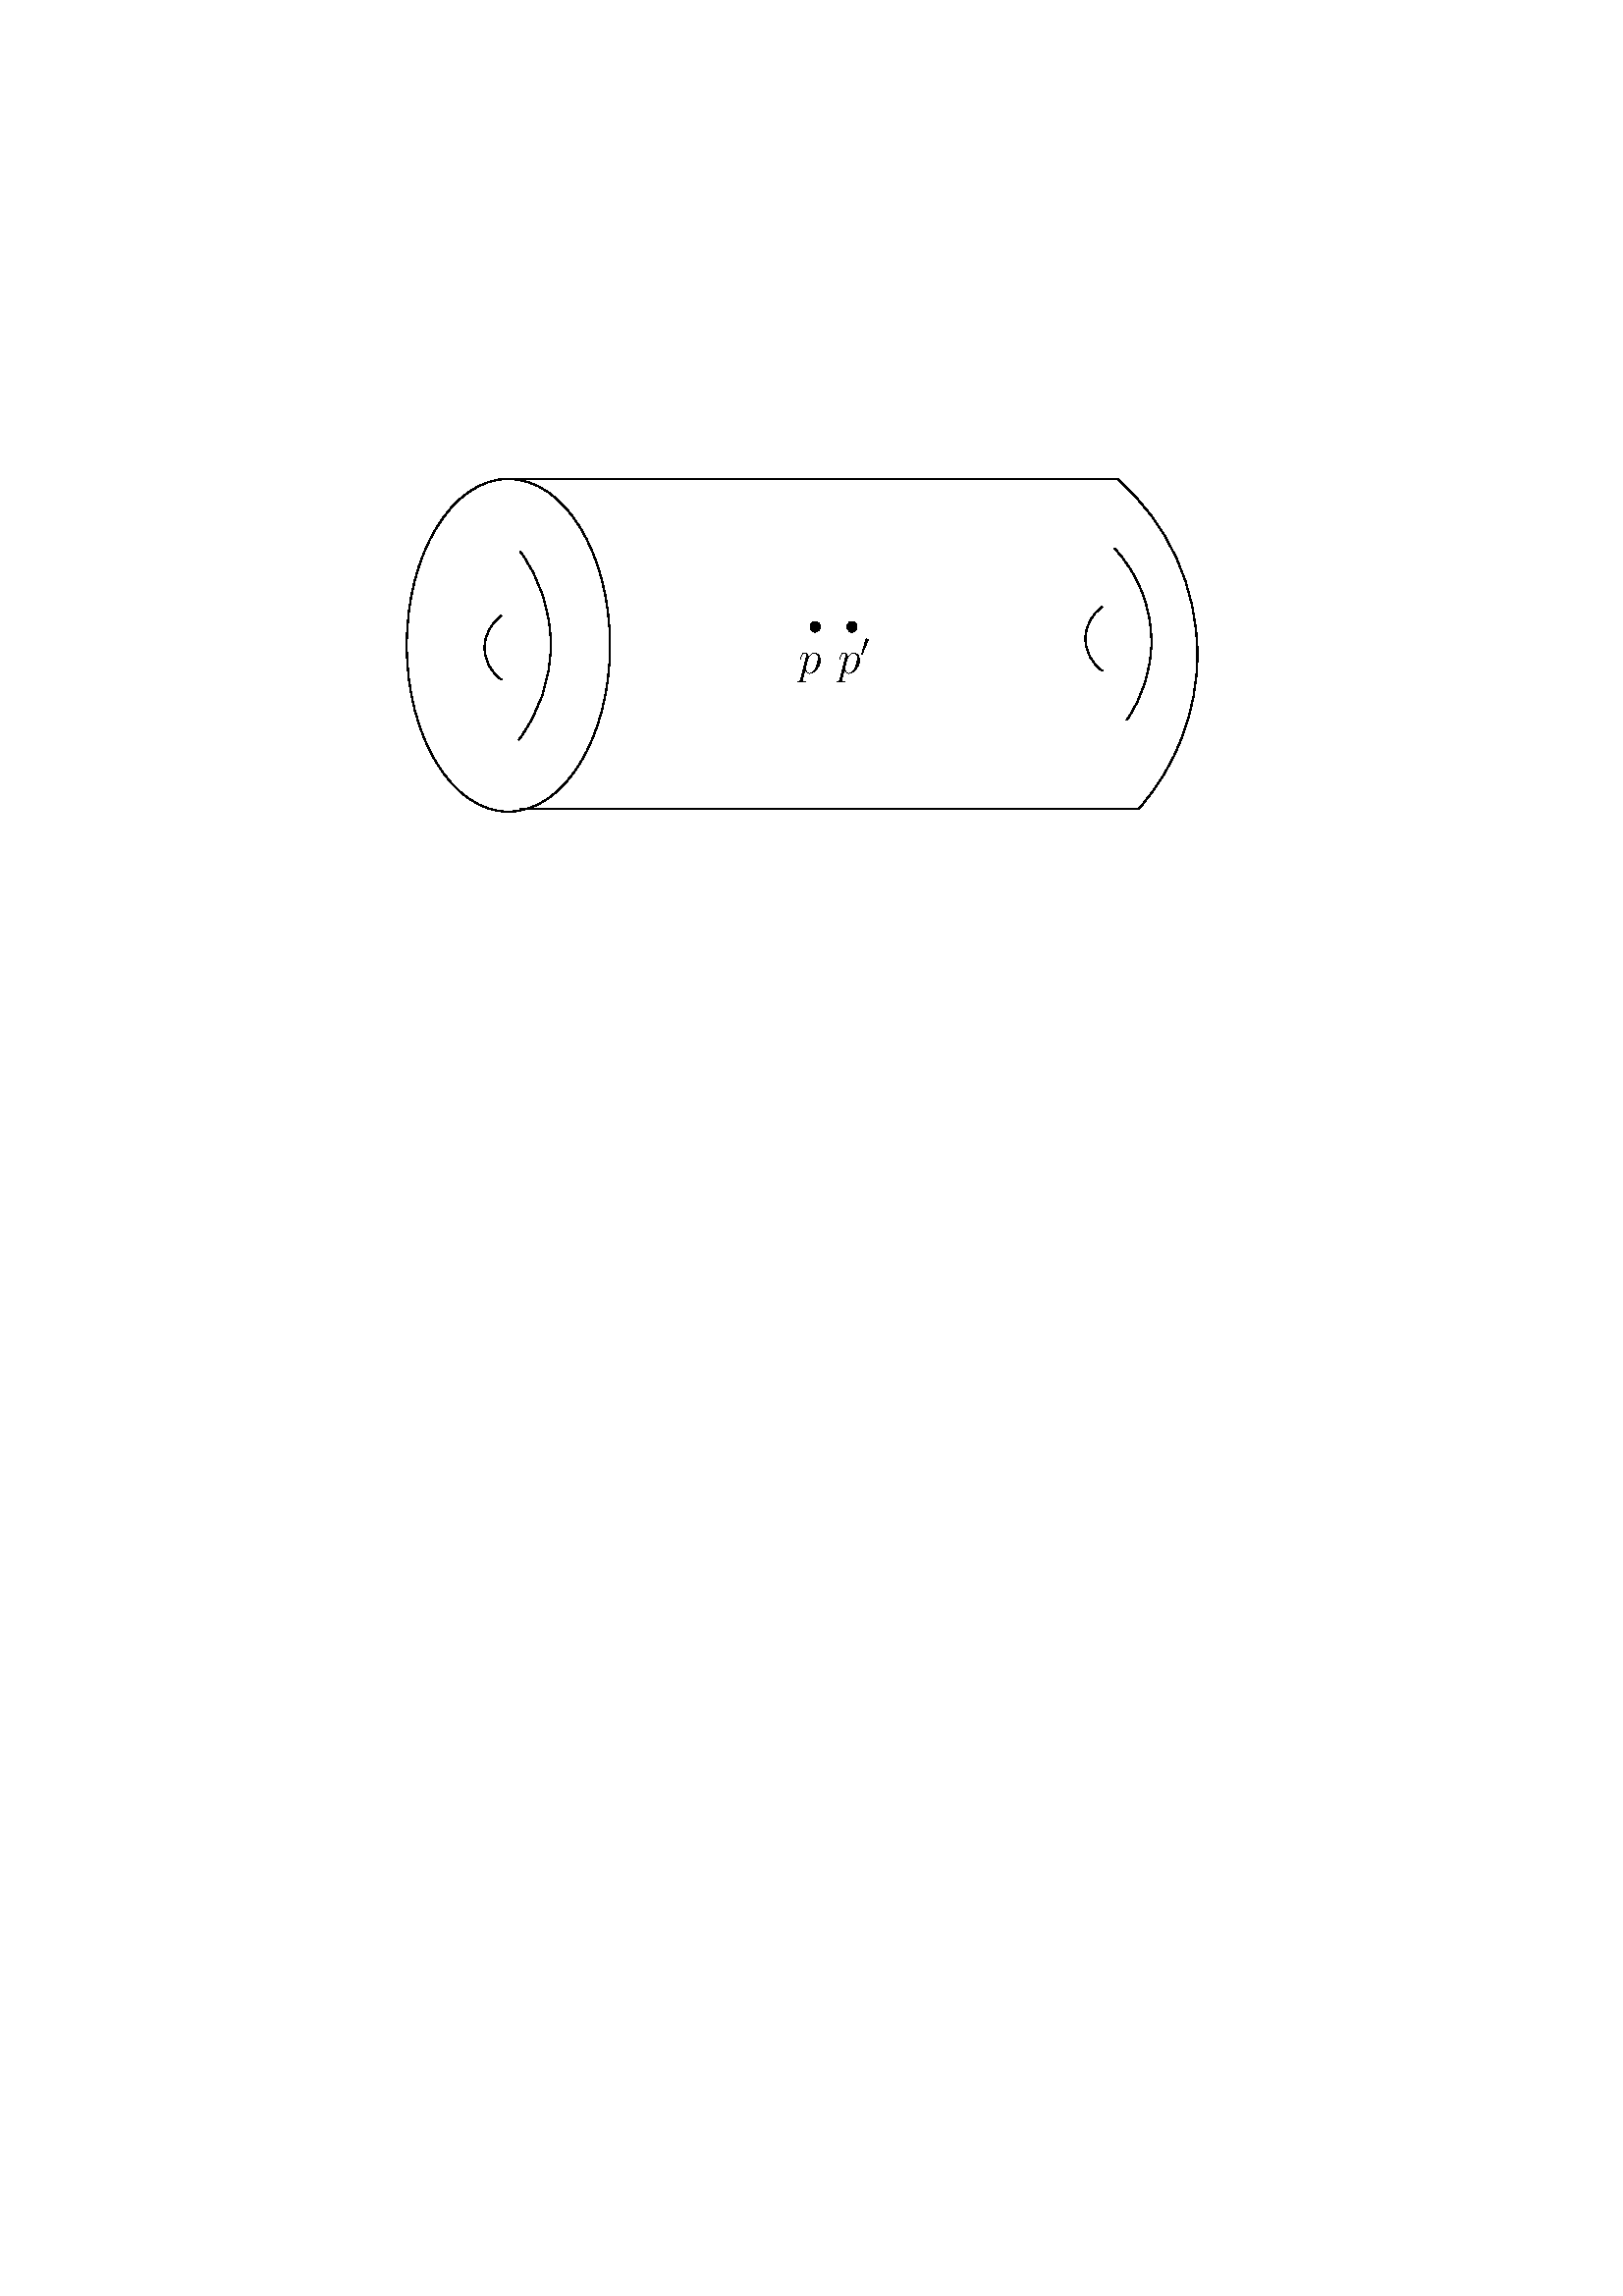
\includegraphics[width=0.75\linewidth]{figures/gla7-9.png}
\caption{A pair of Hecke modifications made at the same value of $z$ but at distinct points in $I$.（原文 Fig.~20）}
\label{fig:xytampo}
\end{figure}

But so far we have not said anything that depends on the
singularity of the weighted projective space. To see its role, let
$^L\negthinspace w=(1/2,-1/2)$ be the weight corresponding to the
two-dimensional representation.  The operator product expansion of
the corresponding Wilson operator with itself should read
% 式 (10.31)
\setcounter{equation}{30}
\begin{equation}\label{eq:murtog}
T({}^L\negthinspace w)\cdot T({}^L\negthinspace
w)=T({}^L\negthinspace\bar w)\oplus T(0),
\end{equation}
 where $0$ is the zero weight,
and $T(0)=1$ is the corresponding trivial 't Hooft operator. (The coefficients are
really one-dimensional vector spaces, but we have omitted them.)  Let
us see how this comes about.  The space of Hecke modifications of
type $^L\negthinspace w$ is isomorphic to $\Bbb{CP}^1$. If
(\xytampo) we make repeated Hecke modifications of type
$^L\negthinspace w$ at the same point $z\in C$ but different
points in $I$, we get a moduli space $\bar\EUZ({}^L\negthinspace
w,z,y;{}^L\negthinspace w,z,y')$ that is a $\Bbb{CP}^1$ bundle
over $\Bbb{CP}^1$.  Its cohomology is four-dimensional, with
classes in dimensions $d=0,2,2,4$, so the eigenvalues of $\EUK$
are $-2,0,0,2$.

Now let us try to take the limit as $y\to y'$. For any $y<y'$, we
can use Hodge theory; the space of harmonic forms on $\bar\EUZ$ is
four-dimensional.  At $y=y'$, an $A_1$ orbifold singularity
develops; the local structure looks like $\Bbb{R}^4/\Bbb{Z}_2$.
For $y$ slightly less than $y'$ (compared to the length of the
interval $I$), this singularity is resolved.  The resolution can
be locally modeled by  a  hyper-Kahler manifold $\EUWW$
(discovered in \cite{ref130}) that in one of its complex structures can be identified
with $T^*\Bbb{CP}^1$. The metric on $\EUWW$ is complete, and
moreover, is asymptotic at infinity to the flat metric on
$\Bbb{R}^4/\Bbb{Z}_2$.

Crucially for us, the space of ${\Bbb{L}}^2$ harmonic forms on
$\EUWW$ is one-dimensional, generated  \cite{ref130}\ by a two-form
$\omega$. (Note that here the ${\Bbb{L}}^2$ condition has to do
with the behavior at infinity, while in the definition of
intersection cohomology it has to do with the behavior near
singularities.) Being in ${\Bbb{L}}^2$, this form has support near
the exceptional divisor, and as $y\to y'$ (and the exceptional
divisor shrinks), it converges to a form with delta function
support at the singularity. Having $d=2$, it corresponds to a
cohomology class with $\EUK=0$, the value corresponding to the
trivial representation of $^L\negthinspace G=SU(2)$. The
${\Bbb{L}}^2$ harmonic two-form on $\EUWW$ exists for topological
reasons that can be understood from arguments in \cite{ref131}.

Now we can understand the meaning of the operator product relation
\eqref{eq:murtog}.  The left hand side is associated with the space
$\bar\EUZ$ of repeated Hecke modifications.  For $y<y'$, it is a
$\Bbb{CP}^1$ bundle over $\Bbb{CP}^1$, and has a four-dimensional
space of harmonic forms, which is the physical Hilbert space
${\cal H}$.  A three-dimensional subspace of this space consists
of harmonic forms that, as $y\to y'$, converge to ${\Bbb{L}}^2$
harmonic forms on the smooth part of
$\bar\EUZ{}^*=\Bbb{WCP}^2(1,1,2)$ (which is the limit of
$\bar\EUZ$ for $y\to y'$). They reflect the contribution of
$T({}^L\negthinspace\bar w)$ to ${\cal H}$. The fourth harmonic
form can be approximated for $y$ near $y'$ by the $\Bbb{L}^2$
harmonic form on $\EUWW$ and is supported near the exceptional
divisor. The support of this fourth harmonic form converges as
$y\to y'$ to the singular point of $\bar\EUZ{}^*$, which is the
space of Hecke modifications of weight $^L\negthinspace w=0$. It
is the contribution of $T(0)$ to ${\cal H}$. The fact that the
coefficient of $T(0)$ is 1 expresses the fact that the space of
harmonic two-forms that converge to the singularity as $y\to y'$
is precisely one-dimensional.  To be more exact, the coefficient of $T(0)$ is
this one-dimensional space of harmonic forms.

More generally, suppose we are given any pair of weights
$^L\negthinspace w$, $^L\negthinspace w'$. We want to describe the
operator product $T({}^L\negthinspace w)\cdot T({}^L\negthinspace
w')$, which is expected to take the form
% 式 (10.32)
\setcounter{equation}{31}
\begin{equation}\label{eq:mitory}
T({}^L\negthinspace w)\cdot T({}^L\negthinspace
w')=T({}^L\negthinspace\,\bar w)\oplus\left(\oplus_{\alpha\in \EUR'}\,N_\alpha
\otimes T({}^L\negthinspace w_\alpha)\right),
\end{equation}
 where $^L\negthinspace\,\bar
w={}^L\negthinspace w+{}^L\negthinspace w'$, and the sum runs over
weights associated to $^L\negthinspace\,\bar w$.   As $y\to y'$,
$\bar\EUZ({}^L\negthinspace w,y,z;{}^L\negthinspace w,y',z)$
converges as a space to $\bar\EUZ({}^L\negthinspace\,\bar w,y,z)$
(whose dependence on $y$ and $z$ is inessential). Some of the
${\Bbb{L}}^2$ harmonic forms on the moduli space converge to such
forms on the smooth part of $\bar\EUZ({}^L\negthinspace\,\bar w)$.
These are the contribution of $T({}^L\negthinspace\,\bar w)$ in
the operator product expansion. Others converge to have delta
function support on $\bar\EUZ({}^L\negthinspace w_\alpha)$ for
some associated weight $^L\negthinspace w_\alpha$ of
$^L\negthinspace\bar w$.  The forms that for $y\to y'$ have
support on $\bar\EUZ({}^L\negthinspace w_\alpha)$ and not on
$\bar\EUZ({}^L\negthinspace w_\beta)$ for any weight
$^L\negthinspace w_\beta$ associated to $^L\negthinspace w_\alpha$
are the contribution of $T({}^L\negthinspace w_\alpha)$ in the
operator product.

Let us simply conclude by describing how this idea has been
expressed mathematically \cite{ref97,ref98}.  The  moduli
space $\bar\EUZ({}^L\negthinspace w,z,y;{}^L\negthinspace
w',z,y')$ is a fibration with fiber $\bar\EUZ ({}^L\negthinspace
w',z,y')$ and base $\bar\EUZ({}^L\negthinspace w,z,y)$, as we
explained in section 第~\ref{sec:kahstr}~节. As $y\to y'$, this moduli space is
``blown down'' to make the more singular space
$\bar\EUZ({}^L\negthinspace\,\bar w,z,y')$, whose dependence on
$z$ and $y'$ is inessential. The blowdown is a rational map
% [WARN] 公式 \eqn\eqref{eq:normo} 无编号或重复
\begin{equation*}
\tag*{(10.33)}
\pi:\bar\EUZ({}^L\negthinspace w,z,y;{}^L\negthinspace
w',z,y')\to \bar\EUZ({}^L\negthinspace\,\bar w).
\end{equation*}

We write $IC({}^L\negthinspace w)\star IC({}^L\negthinspace w')$
for the standard intersection cohomology complex on
$\bar\EUZ({}^L\negthinspace w,z,y;{}^L\negthinspace w',z,y')$.
(The notation is motivated by the fiber bundle structure of this
space.)  There is a pushdown map $\pi_*$ in intersection
cohomology.  As the sheaf $IC({}^L\negthinspace w)\star
IC({}^L\negthinspace w')$ is invariant under the group called
$GL(N,{\cal O})$ in section 第~\ref{sec:affgrass}~节\ or its analog $G({\cal O})$
for other $G$, and $\pi_*$ commutes with this action, the pushdown
$\pi_*(IC({}^L\negthinspace w)\star IC({}^L\negthinspace w'))$ is
likewise invariant under $G({\cal O})$.  It therefore is possible
to expand it as a sum of the standard intersection cohomology
complex $IC({}^L\negthinspace\bar w)$ of
$\bar\EUZ({}^L\negthinspace\bar w)$, and the complexes
$IC({}^L\negthinspace w_\alpha)$ that are supported on the
singular orbits with weights $^L\negthinspace w_\alpha$ that are
associated to $^L\negthinspace\bar w$.  (These are the only
$G({\cal O})$-invariant intersection cohomology complexes on
$\bar\EUZ({}^L\negthinspace\bar w)$.)

So we must have\footnote{We have shifted all complexes in dimension to
be symmetric between positive and negative dimensions.  The map
$\pi_*$ preserves this symmetry.  So we do not need to be
concerned about further shifts.}
% 式 (10.34)
\setcounter{equation}{33}
\begin{equation}\label{eq:yrox}
\pi_*\left(IC({}^L\negthinspace w)\star
IC({}^L\negthinspace w')\right)=IC({}^L\negthinspace\bar
w)\oplus \left(\bigoplus_\alpha\, \tilde N_\alpha \otimes \,IC({}^L\negthinspace w_\alpha)\right).
\end{equation}
 The
``coefficient'' of the leading term $IC({}^L\negthinspace\bar w)$ is
a trivial one-dimensional vector space (which we can omit),
since the map $\pi$ is an isomorphism over the smooth part of
the moduli space. The nature of the leading term has an elementary
explanation explained in the discussion of eqn. \eqref{eq:hffo}. The other
``coefficients'' are vector spaces $\tilde N_\alpha$. This formulation is analogous to the
general structure \eqref{eq:hffo}\ or \eqref{eq:zurgo}\ of the product of 't Hooft
operators, with the intersection complex $IC({}^L\negthinspace
w_\alpha)$ representing the contribution of the 't Hooft operator
$T({}^L\negthinspace w_\alpha)$.  Of course, the hard part of the
proofs \cite{ref97,ref98} is to describe the spaces $\tilde N_\alpha$ and
establish their isomorphism with the analogous spaces $N_\alpha$ that appear in \eqref{eq:omigron}.
